\section{TÍCH CỦA VECTƠ VỚI MỘT SỐ THỰC}
\subsection{TÓM TẮT LÝ THUYẾT}
\subsubsection{Định nghĩa}
Cho số thực $k \ne 0$ và $\overrightarrow{a} \ne \vec{0}$.
\begin{center}
	\begin{minipage}[b]{8cm}
		\begin{tcolorbox}[colframe=orange,colback=white,boxrule=0.2mm]
			Tích của vec tơ $\overrightarrow{a}$ với số thực $k>0$ là một vec tơ, kí hiệu $k\overrightarrow{a}$, \indamm{cùng hướng} với $\overrightarrow{a}$ và có đồ dài bằng $k \big|\vec{a}\big|$
		\end{tcolorbox}
	\end{minipage}\hspace{1cm}
	\begin{minipage}[b]{8cm}
		\begin{tcolorbox}[colframe=orange,colback=white,boxrule=0.2mm]
			Tích của vec tơ $\overrightarrow{a}$ với số thực $k<0$ là một vec tơ, kí hiệu $k\overrightarrow{a}$, \indamm{ngược hướng} với $\overrightarrow{a}$ và có đồ dài bằng $\big|k\big|\cdot \big|\vec{a}\big|$
		\end{tcolorbox}
	\end{minipage}
\end{center}
\immini{\indamm{ Ví dụ:} Theo hình vẽ bên, thì $\overrightarrow{b}=3\overrightarrow{a}$; $\overrightarrow{c}=-2\overrightarrow{a}$; $\overrightarrow{c}=-\dfrac{2}{3}\overrightarrow{b}$.
	\begin{luuy}
		Quy ước: $0 \cdot \overrightarrow{a}=\overrightarrow{0}$.
	\end{luuy}
}{
	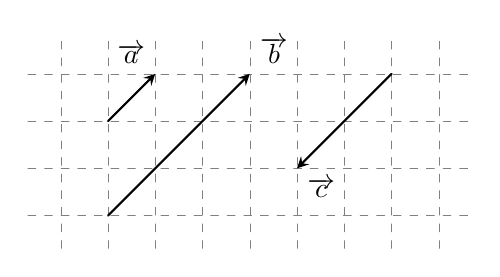
\begin{tikzpicture}[>=stealth,scale=0.6, line join=round, line cap=round]
		\draw[line width=0.05pt,gray,dashed] (-0.7,-0.7) grid (8.7,3.7);
		\draw[->,thick](1,2)--(2,3)node[above left]{$\overrightarrow{a}$};
		\draw[->,thick](1,0)--(4,3)node[above right]{$\overrightarrow{b}$};
		\draw[->,thick](7,3)--(5,1)node[below right]{$\overrightarrow{c}$};
\end{tikzpicture}}

\subsubsection{Điều kiện để hai vectơ cùng phương}
 \begin{gachsoc}
 	\begin{itemize}
 		\item [\ding{172}] Điều kiện cần và đủ để $\overrightarrow{a}$ và $\overrightarrow{b} \ne \overrightarrow{0}$ cùng phương là có một số thực $k$ để $\overrightarrow{a}=k\overrightarrow{b}$.
 		\item [\ding{173}] Ba điểm phân biệt $A$, $B$, $C$ thẳng hàng khi có số thực $k$ để $\overrightarrow{AB}=k\overrightarrow{AC}$.
 	\end{itemize}
 \end{gachsoc}
\subsubsection{Tính chất}
\begin{tcolorbox}[colframe=orange,colback=white,boxrule=0.2mm]
	Với hai vec tơ $\vec{a}$, $\vec{b}$ và hai số thực $k$, $t$ ta luôn có
	\begin{listEX}[3]
		\item [$\bullet$] $k(t\vec{a})=(k \cdot t)\vec{a}$.
		\item [$\bullet$] $(k+t)\vec{a}=k\vec{a}+t\vec{a}$.
		\item [$\bullet$] $k(\vec{a}+\vec{b})=k\vec{a}+k\vec{b}$.
		\item [$\bullet$] $k(\vec{a}-\vec{b})=k\vec{a}-k\vec{b}$.
		\item [$\bullet$] $1\cdot \vec{a})=\vec{a}$. 
		\item [$\bullet$] $(-1)\cdot \vec{a})=-\vec{a}$.
	\end{listEX}
\end{tcolorbox}
\subsubsection{Phân tích một vectơ theo hai vectơ không cùng phương}
\begin{gachsoc}
	\immini{Cho hai vectơ $\vec{a}$ và $\vec{b}$ không cùng phương. Khi đó mọi vectơ $\vec{c}$ đều phân tích được một cách duy nhất theo hai vectơ $\vec{a}$ và $\vec{b}$, nghĩa là có duy nhất cặp số $h,k$ sao cho $\vec{c}=h\vec{a}+k\vec{b}$
		\begin{itemize}
			\item [$\bullet$] Theo quy tắc hình bình hành, ta có $$\overrightarrow{c}=\overrightarrow{OH}+\overrightarrow{OK}$$
			\item [$\bullet$] Giả sử $\overrightarrow{OH}= h\overrightarrow{a}$ và $\overrightarrow{OK}= k\overrightarrow{b}$ thì $\vec{c}=h\vec{a}+k\vec{b}$.
		\end{itemize}
	}{
	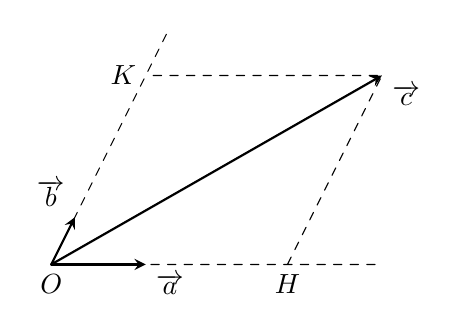
\begin{tikzpicture}[>=stealth,scale=0.6, line join=round, line cap=round]
	%\draw[line width=0.05pt,gray,dashed] (-0.7,-0.7) grid (8.7,4.7);
	\draw[->,thick](0,0)--(0.5,1)node[above left]{$\overrightarrow{b}$};
	\draw[->,thick](0,0)--(2,0)node[below right]{$\overrightarrow{a}$};
	\draw[->,thick](0,0)--(7,4)node[below right]{$\overrightarrow{c}$};
	\draw[dashed](0,0)--(7,0) (0,0)--(2.5,5) (5,0)--(7,4)--(2,4);
	\node[below] at (5,0) {$H$};
	\node[below] at (0,0) {$O$};
	\node[left] at (2,4) {$K$};
	\end{tikzpicture}}
\end{gachsoc}

\begin{enumerate}[\faPencilSquareO]
	\item Muốn so sánh được 2 vectơ theo một tỉ số $k \ne 0$ tương ứng thì giá của hai véc tơ đó phải song song hoặc trùng nhau.
	\item Xét hai vec tơ cùng phương $\overrightarrow{AB}$ và $\overrightarrow{CD}$.
	\begin{itemize}
		\item Bước 1. Tính tỉ lệ đoạn thẳng $\dfrac{AB}{CD}=m$.
		\item Bước 2. Xem xét, nếu
		\begin{itemize}
			\item $\overrightarrow{AB}$ cùng hướng với $\overrightarrow{CD}$ thì $\overrightarrow{AB}=m\overrightarrow{CD}$.
			\item $\overrightarrow{AB}$ ngược hướng với $\overrightarrow{CD}$ thì $\overrightarrow{AB}=-m\overrightarrow{CD}$.
		\end{itemize}
	\end{itemize}
\end{enumerate}

[$\bullet$] So sánh hai vectơ theo tỉ số $k$ tương ứng
\begin{enumerate}[\faPencilSquareO]
	\item Muốn so sánh được 2 vectơ theo một tỉ số $k \ne 0$ tương ứng thì giá của hai véc tơ đó phải song song hoặc trùng nhau.
	\item Xét hai vec tơ cùng phương $\overrightarrow{AB}$ và $\overrightarrow{CD}$.
	\begin{itemize}
		\item Bước 1. Tính tỉ lệ đoạn thẳng $\dfrac{AB}{CD}=m$.
		\item Bước 2. Xem xét, nếu
		\begin{itemize}
			\item $\overrightarrow{AB}$ cùng hướng với $\overrightarrow{CD}$ thì $\overrightarrow{AB}=m\overrightarrow{CD}$.
			\item $\overrightarrow{AB}$ ngược hướng với $\overrightarrow{CD}$ thì $\overrightarrow{AB}=-m\overrightarrow{CD}$.
		\end{itemize}
	\end{itemize}
\end{enumerate}